\documentclass[10pt,journal]{IEEEtran}

\ifCLASSOPTIONcompsoc
  % IEEE Computer Society needs nocompress option
  % requires cite.sty v4.0 or later (November 2003)
  \usepackage[nocompress]{cite}
\else
  % normal IEEE
  \usepackage{cite}
\fi

\usepackage{amsmath,amssymb,amsfonts}
\usepackage{algorithmic}
\usepackage{graphicx}
\usepackage{textcomp}
\usepackage{xcolor}

\hyphenation{op-tical net-works semi-conduc-tor}

\def\BibTeX{{\rm B\kern-.05em{\sc i\kern-.025em b}\kern-.08em
		T\kern-.1667em\lower.7ex\hbox{E}\kern-.125emX}}

\makeatletter
\def\endthebibliography{%
	\def\@noitemerr{\@latex@warning{Empty `thebibliography' environment}}%
	\endlist
}
\makeatother

\makeatletter
\newcommand*\titleheader[1]{\gdef\@titleheader{#1}}
\AtBeginDocument{%
	\let\st@red@title\@title
	\def\@title{%
		\bgroup\normalfont\large\centering\@titleheader\par\egroup
		\vskip1em\st@red@title}
}
\makeatother


\begin{document}
\bstctlcite{IEEEexample:BSTcontrol}

\title{Parallel Patterns with C and OpenMP}


\author{
	{
		Filipe~de Luna,~\IEEEmembership{48425} and
        Gabriel Batista,~\IEEEmembership{47590}
    } \\ Department of Informatics - FCT-NOVA
        
}

\markboth{Concurrency and Parallelism - DI FCT-UNL, 2019-2020}%
{Concurrency and Parallelism - DI FCT-UNL, 2019-2020}

% make the title area
\maketitle

\section{Introduction}
For the Concurrency and Parallelism course of the Integrated Masters in Computer Science at FCT-NOVA, we were asked to implement a series of parallel patterns using the \textit{OpenMP} API. The following document describes our implementation of these patterns, the results we’ve achieved during the testing phase and our interpretation of these same results.

We developed the project in a \textit{Linux} environment using \textit{C}, the \textit{GCC} compiler and \textit{CMake} for building. We used the standard \textit{GNU} argument parser (argp) \cite{argp}. This made testing a lot easier, allowing us to add flags and arguments to our program.

Our most important tool was \textit{OpenMP} \cite{omp}, a multi-platform API that allows the user to add pragmas to programming blocks in order to parallelize code. The main perk of \textit{OpenMP} is that parallel code ends up looking extremely similar to serial code, making code much more readable and still allowing serial execution.

We have created two python scripts to aid us in testing. The first script, named “tester”, runs the program several times with the appropriate flags and saves the results. The tester can be configured to run a specific algorithm or all with a set of numbers of jobs, number of threads and, lastly, the number of repetitions for every test/number of jobs/thread combo, from which we extract a mean value. All these results are written to a file of our choosing.

The tester also allowed for configuring tests to run with different sets of numbers of jobs, since some algorithms run a lot faster than others and we needed to keep overall testing times low.  Another parameter, was “weight”, which activated a flag in the program that added a for loop with a configurable number of iterations to every worker. We tested all our worker-based patterns with a weight of 250 iterations. Ideally, we would increase the number of total jobs, but this wasn't really viable as the worker was really light and for the number of needed jobs, it would result in running out of RAM. This was necessary since some algorithms had a very significant management cost and it allowed us to simulate a heavier work load in order to visualize their gains more accurately. 

The second python script, the “grapher”, reads the output file with the results and creates a graph, using Matplotlib \cite{matplotlib}, for each test, in order to help us visualize the data. 

Since our computers had a limited core count, we couldn’t get a realistic perception of the gains that the parallelization of these patterns could allow for. So we ran our tests in the cluster maintained by our Faculty’s Department of Informatics. The particular node we used for tests had 64 cores. 

For profiling we ran the \textit{CLion} default profiler (\textit{perf} on our Linux systems) on a machine with 16 threads (8 physical + 8 logical). Profiling was incredibly useful to get an idea of how much the management cost was, and how much time was spent doing serial work.

To get realistic results for each thread count, we disabled \textit{OpenMP's} default dynamic scheduling and forced it to \textit{static}. This means that the number of threads we specified will actually be used, instead of \textit{OpenMP} dynamically optimizing the thread count for the given workload, which is necessary in order to obtain accurate and deterministic results.

\section{Mandatory Parallel Patterns}

% Map --------------------------------------------------------------	
\subsection{The Map Pattern}
\label{map}

\subsubsection{Implementation}

The Map pattern was the simplest and most straightforward to implement as we can use \textit{OpenMP's} \textit{for} construct to map $ n $ jobs to a for loop with $ n $ iterations. This for loop will then be proportionally sliced with each thread receiving a similar slice. Since there are no dependencies between jobs or a necessary order of execution, this algorithm becomes embarrassingly parallelizeable \cite{mccool}.

\subsubsection{Testing}

With 10.000 jobs, the algorithm showed a linear speedup up to 4 cores, with the speedup severely lowering when 8 were used. With upwards of 8 cores, we saw similar linear negative speedup, since the management cost for the creation of these threads was more than the time the threads actually ran their work. Only at 500.000 jobs did the algorithm start showing the expected linear speedup  up to the number of physical threads of the machine (64).

With an added weight of 1000 for iterations, it's possible to observe, on the profiler, that the program spends ~93\% of the time running in parallel. By removing the added weight, we see a drop to ~68\% (the rest being managament cost). It's easy to conclude that the necessary workload per job for the pattern to become viable is not that big, as a for with 1000 iterations is an extremely fast computation in a modern chip.

% Reduce --------------------------------------------------------------		
\subsection{The Reduce Pattern}
\label{reduce}

\subsubsection{Implementation}

Although \textit{OpenMP} includes a reduction construct and can efficiently parallelize reductions, this only works for scalar values and arithmetic operations \cite{ompreduct}. Since we want to create a generic reduction, we had to implement a custom algorithm. The algorithm was based on the 2-phase reduction found McCool's book \cite{mccool}. In the first phase, each thread gets a similar portion of the total work and reduces it (much like a map), and in the second phase, those results are reduced serially. 

\subsubsection{Testing}

As expected, this algorithm showed results very similar to the ones from map (\ref{map}), as it behaved very similarly. Even though the second phase is serial, it only has a maximum of jobs equal to the number of threads, meaning it won't scale significantly and shouldn't affect the gains much. Since the computational weight of the serial computation is not significant, as mentioned earlier, the profiling also showed similar results to map (\ref{map}).

% Scan --------------------------------------------------------------		
\subsection{The Scan Pattern}
\label{scan}

\subsubsection{Implementation}

This pattern was the most complicated to implement of all the mandatory ones. There were many possibilities but we decided on the inclusive three-phase algorithm shown on McCool's book on chapter 5.5 \cite{mccool}. The first two-phases are almost identical to the reduce pattern mentioned earlier in reduce (\ref{reduce}), with the third one using their result of the first value of each slice to compute the following values. Like in reduce, the second phase is serial and has as many computations as the amount of threads executing the algorithm. 

An exclusive scan was created which was just a call to this function which basically does an inclusive scan with an offset of 1, so the first value is 0, and $ n - 1 $ jobs.

\subsubsection{Testing}

The scan did not show improvements switching from 1 to 2 threads in every number of jobs, with the added management costs being higher than the gains up to 1.000.000 jobs. But from upwards of 2 threads, the gains were linear up to 32 threads, with very small improvement from 32 to 64 threads. The reason behind this is due to the fact that this implementation uses $ n - 1 $ threads for the first cycle and the second cycle is serial. This means that, with 2 threads, 2 out of 3 phases are executed serially, with the added management cost not making it worth the extra parallelism in the last phase.

The profiling showed similar results to map (\ref{map}). With the expected parallelism with 2 threads, as mentioned in the last paragraph, resulting in only the expected 33\%. We conclude this algorithm is not a good solution for very low thread counts.

The scan was actually one of the algorithms that ended up showing better results with a higher thread count than the physical cores on the machine. This a phenomenon McCool describes as "Parallel Slack" \cite{mccool}, which ends up giving more flexibility to \textit{OpenMP}, as it can better distribute these chunks of jobs per threads as it sees fit. If there were as many chunks as threads, one hanging thread could hang the entire program.

% Pack -------------------------------------------------------------	
\subsection{The Pack Pattern}
\subsubsection{Implementation}
\label{pack}

Even though we studied pack on McCool's book \cite{mccool}, most of our ideas came from his article on \textit{Dr. Dobb's} \cite{dobbpack}. The main idea is that pack is not a fundamental pattern, meaning it can be implemented by combining others. 

We chose to do an exclusive scan on the filter so that the resulting array would give us the correct position in the destiny array for each item of the source array that is allowed in the filter. We then run a map on the source array, and for each position we check if it is allowed in the filter and, if so, we send it to the position given by the scanned filter array.

\subsubsection{Testing}

To test pack, we created a filter array with the same size as the number of jobs. This array had alternating ones and zeros. On first inspection, pack results seem, really odd, as its performance deteriorated with a growing core up to around 500.000 jobs. And, even between 500.000 and 1.000.000 jobs, it showed a linear speed up from 2 to 8 cores and then started showing a linear negative speedup.

This is due to pack not using a worker, but a \textit{memcpy} instruction that is only executed $ n / 2 $ times, with $ n $ jobs, meaning not only is it not affected by the weight, but also has a much lighter computation. Even though it uses a scan, its worker is custom and does not include weight. This results in much faster computation than other algorithms, until now, for the same job size. It only starts showing the expected linear speedup up to 32 threads at around 5.000.000 jobs with performance deteriorating at 64 but improving again at 128, due to parallel slack.

% Gather --------------------------------------------------------------	
\subsection{The Gather Pattern}
\label{gather}

\subsubsection{Implementation}

Gather's implementation was very similar to pack's (\ref{pack}), with a \textit{memcpy} instruction and a map. The gather was based on the ideas in \textit{Dr. Dobb's} that "a gather is a parallel read of elements of memory that subsequently writes said values to another array according to a filter" \cite{dobbgather}. This filter holds the position in the source array of the element to write for each position, with each index $ i $ of the filter mapping to the same index $ i $ of the destiny array.

\subsubsection{Testing}

For testing, we created a filter with a size of $ n $ and populated it with random integers that could be anywhere between 0 and $ n - 1 $, with $ n $ being the number of jobs.

As expected, the results were basically the same as pack's (\ref{pack}). Gather does execute a \textit{memcpy} always instead of pack's conditional, but the amount of jobs (or job size, as \textit{memcpy} writes in blocks) necessary to see a difference from this verification is immense as \textit{memcpy} is incredibly fast for byte-sized copies.

% Scatter --------------------------------------------------------------	
\subsection{The Scatter Pattern}
\label{scatter}

\subsubsection{Implementation}

Our default implementation of scatter is the atomic scatter. Since it is only briefly mentioned in McCool's book \cite{mccool}, we had to come up with our own solution. We found this variation of scatter particularly hard to implement due to not being able to use \textit{OpenMP's} \textit{atomic} pragma, as it does not work with \textit{memcpy}. Since \textit{memcpy} writes data block by block, two parallel writes can cause a corruption, as the destiny can have part of the information from the first job and part from the second.

Our solution was to use a custom quick-sort that ordered the filter and reflected that order on the source array. By doing so, it was possible to add a conditional \textit{critical} pragma when the next value in the filter is equal to the current. This results in a very heavy reduction of the use of the \textit{critical} pragma and a good parallel performance at the cost of the initial quick-sort computation.

\subsubsection{Testing}

The added quick-sort at the beginning turned this algorithm from $ O(n) $ into $ O(n\log_n) $, meaning the computation needed to be really intense in the parallel phase to make up for the added overhead. We made it possible to set the size of the destiny array. The probability of triggering a critical section is $ 1 / n $, with $ n $ destiny positions. But this does not mean $ 1 - 1 / n $ of the original speed, because the \textit{critical} section halts all the threads, and more halted threads result in more halted work and more management cost to halt and get back to work.  This is also called "lock management overhead", which increases with the number of threads \cite{lockmanage} 

With a low destiny array of just 10 positions, we only managed a parallelization of around 5\% because we kept hitting the \textit{critical} section. After changing the destiny array size to $ n / 50 $, with $ n $ jobs, the profiler showed around 80\% parallelization time, due to hitting the \textit{critical} section much less. Since running with only 10 positions in the destiny array resulted in so many collisions, we also had to run a lower number of jobs and the resulting speedups weren't satisfactory as it only showed a significant speedup starting at 50.000 iterations and only up to 8 threads. After 8 threads, the effects of the \textit{critical} section overcame the added parallelization. With $ n / 50 $ positions in the destiny array, the algorithm ran a lot faster, but the speedup was relatively similar. 

We conclude this algorithm does work but does not scale well at all, as its performance is completely tied to the size of the destiny array.

% Pipeline --------------------------------------------------------------	
\subsection{The Pipeline Pattern}
\subsubsection{Implementation}

The pipeline is an algorithm that does a collection of operations on a series of data, in order. The default pipeline implementation we chose was the map pipeline briefly discussed on McCool's book \cite{mccool}. This algorithm is just a succession of maps, with each map traversing all the data and executing the respective operation.

\subsubsection{Testing}

Since this algorithm relies on maps, which are embarrassingly parallel, it comes as no surprise that the profiler confirms this, with over 80\% of the time running in parallel. For testing, a group of three workers were chosen that: multiplied the value by two, incremented and then divided the result by two.

The speedup was pretty linear until the number of physical threads was reached, showing a little more improvement with 128 threads due to the parallel slack phenomenon mentioned earlier in scan (\ref{scan}). However, the algorithm only started showing consistent results starting with 100.000 iterations, meaning this is when the gains obtained from parallelizing obfuscate the management cost.

% Farm --------------------------------------------------------------	
\subsection{The Farm Pattern}
\subsubsection{Implementation}

The farm pattern is very hard to implement in \textit{OpenMP}, since we can't have a fine-grained control of threads, as \textit{OpenMP} dynamically distributes and hands work to threads. We can ask \textit{OpenMP} to use $ n $ threads in a computation, but we can't choose which threads will be used, and controlling them is hard.

\textit{OpenMP} contains a \textit{task} pragma that is an implementation of a farm pattern \cite{jlfarm}. With \textit{task} we can add computational tasks to a queue from which \textit{OpenMP} will dynamically distribute throughout all the threads however it sees fit.

This is the implementation we went for. For each job we create a task and \textit{OpenMP} distributes it through the number of threads we set. The loop that creates all the tasks needs to be executed by a single thread who acts as a master, and afterwards becomes a slave, joining all the other threads in consuming these tasks.

\subsubsection{Testing}

With an added weight of 250 iterations, we saw a linear negative speedup as we increased the number of threads, throughout all the numbers of iterations. With the weight increased to 15.000 iterations, we could observe a linear speedup up to 16 cores. With upwards of 16 cores, the speedup would exponentially grow negatively, with 64 threads being slower than one. But, in the case of 128 threads, it lowers the time exponentially and is almost at its fastest.

The culprit of this odd phenomenon was \textit{OpenMP} itself, as it increases the time to create a task as more threads are used \cite{granularity}. Another interesting feature is "task throttling", an internal mechanism in \textit{OpenMP} that forces \textit{task} serialization after a specific number of \textit{tasks} have been created \cite{granularity}. As to why using 128 threads results in an incredible speedup, we believe it is attributed to the fact that, besides the expected parallel slack, increasing the number of threads also increases the maximum number of simultaneous tasks before throttling.

Since this implementation has little to no significant serial work, we expect it to be embarrassingly parallel. We confirm this when we run the profiler and consistently upwards of 90\% of the time in parallel work. We can conclude that \textit{OpenMP} isn't suited to implement farm as tasks come with a heavy management cost and its usage isn't always deterministic. 

\section{Extra Parallel Patterns}

% Priority Scatter --------------------------------------------------------------	
\subsection{The Priority Scatter Pattern}
\subsubsection{Implementation}

In this version of scatter briefly discussed in the book \cite{mccool}, the order of the job dictates its priority. It also does not take into account collisions, as subsequent writes will overwrite previous data and yield a deterministic result based on the order \cite{mccool}.

The implementation of this pattern was pretty straightforward as it's essentially an \textit{OpenMP} \textit{for} construct with an \textit{ordered} construct, forcing it to execute the iterations in order \cite{omporder}.

\subsubsection{Testing}

This pattern shows consistently worse performance for all numbers of jobs, as the number of threads increases, up to 1.000.000 iterations. We can attribute this to the fact that it shares the same issue as gather \ref{gather}: \textit{memcpy} is too fast and we need an extreme number of jobs to make up for the management cost. As expected, if we add a for loop with 1000 iterations, the management cost stops being relevant and we get a continuous linear speedup up to the number of physical cores. 

% Item-Bound Pipeline --------------------------------------------------------------	
\subsection{The Item-Bound Pipeline Pattern}
\label{itembound}

\subsubsection{Implementation}

This the pipeline implementation was based on slides from the University of Oregon \cite{pipelineoregon}. It's item-bound nature basically means a thread takes a job and executes all the workers at once on it, taking advantage of data locality. The implementation is pretty straightforward as it is basically an \textit{OpenMP} \textit{for} construct that, at each job, executes all the workers.

\subsubsection{Testing}

As expected, this algorithm is embarrassingly parallel, with the profiler reporting around over 90\% time spent in parallel computations and shows a linear speedup up to 32 threads and a smaller speedup up to 128, due to parallel slack.

% Serial Pipeline --------------------------------------------------------------	
\subsection{The Serial Pipeline Pattern}

\begin{figure}[htbp]
	\centerline{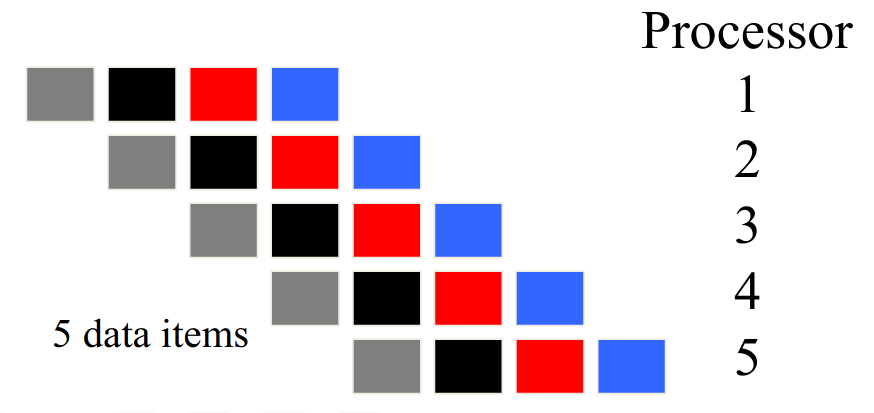
\includegraphics[scale=0.12]{img/serialpipeline.png}}
	\caption{ A serial pipeline. Source: \cite{pipelineoregon}.  }
	\label{serialpipe}
\end{figure}

\subsubsection{Implementation}

Like the item-bound pipeline (\ref{itembound}), this implementation was based on slides from the University of Oregon \cite{pipelineoregon}. The main purpose of this algorithm is to allow for various workers, that cannot be parallelized, to run through a parallel pipeline. 

As seen on figure \ref{serialpipe}, it starts executing worker $ i $ on a job after worker $ i - 1 $ was executed on the previous job. This means that, for the first and last $ n - 1 $ cycles, with $ n $ workers, it won't be able to make full use of it's parallelization potential. Another problem with this pipeline is that it only makes sense to have as many threads as there are workers, as the number of workers dictates the maximum parallelization.

The implementation is basically a for loop with an \textit{OpenMP} \textit{for} construct inside. The outer for accounts for the amount of steps the total algorithm takes from the first job's first worker to the last job's last worker. The inner \textit{for} construct does runs the expected worker in each data for this step.

\subsubsection{Testing}

The number of workers were set to 64 (the number of physical threads on the machine). Since the number of jobs is much larger than the number of workers, the first and last $ n - 1 $ cycles, mentioned earlier, won't make much of a difference. The large number of workers makes this algorithm take a lot of time since, not only is the amount of work multiplied by the amount of workers, but also each worker has the inherent weight. So, to account for this, we executed less total jobs.

With the default weight of 250 iterations, there was an acceptable linear speedup up to 8 threads, with improvement starting at 500 jobs and going up to 10.000. After raising the weight of the workers to 10.000 iterations, the tests showed the expected linear speedup all the way to the number of threads on the machine (64). We can conclude the necessity for such a high weight in a job, to make up for the management cost, is because, since the \textit{OpenMP's} \textit{parallel} construct is inside a for loop, the loop multiplies the management cost by its iterations.

% Stencil --------------------------------------------------------------	
\subsection{The Stencil Pattern}

\subsubsection{Implementation}

This implementation was based on the one demonstrated in chapter 7.1 of McCool's book \cite{mccool}. Stencil is similar to a map, but every job is computed from the result of the reduction of value $ i - n $ to $ i + n $, with $ i $ being the job and $ n $ the radius of the vicinity to be computed. It's a technique that is used in image manipulation software, for instance, so that a pixel gets a color that is the average of the pixels around it.

The implementation was straightforward as it is essentially a map, but instead of just doing it's respective worker, it creates a temporary variable to hold the reduction and, after computing this reduction, stores the value in its respective place of the destiny array.

\subsubsection{Testing}

For testing, we set the number of jobs in the vicinity to be computed to 5. This means that, unless we're at an edge, we reduce 11 jobs for each job, which results in a lot more computations for each job. To account for this, less total jobs were ran. 

At 50.000 jobs, the cost of management was compensated for and it was possible to observe an almost linear speedup up to the number of physical threads in the machine (64). Since this algorithm is a variation of a map, it's also embarrassingly parallel, with the profiler showing over 90\% of the time is spent in parallel computation.

% Parallel Prefix --------------------------------------------------------------	
\subsection{The Parallel-Prefix Algorithm}

\begin{figure}[htbp]
	\centerline{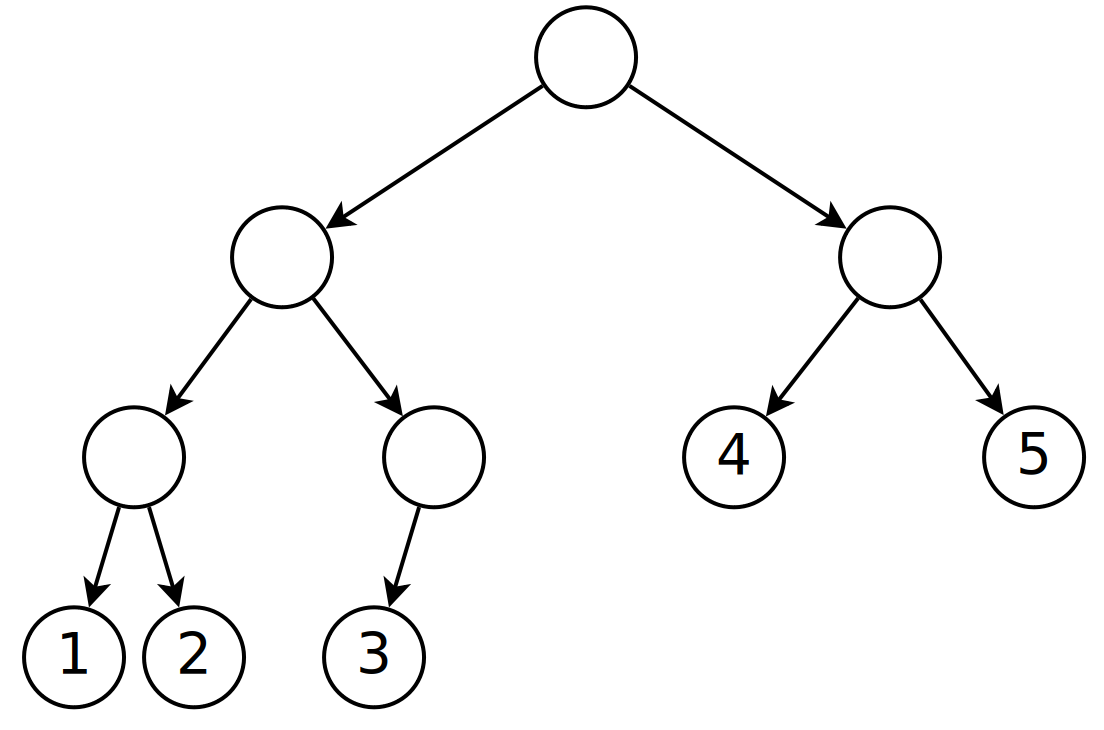
\includegraphics[scale=0.10]{img/parprefix.png}}
	\caption{ Our Parallel-Prefix implementation.  }
	\label{parprefixpic}
\end{figure}

\subsubsection{Implementation}

The parallel-prefix is an algorithm that implements the scan pattern. Our implementation was based on the slides by David Walker from Princeton University \cite{parprefix}. It maps an array of jobs to the bottom of a tree and does two passes - one up pass and one down pass. The first pass computes the result of the computations bottom-up, while the second one traverses the tree top-down to compute the prefixes - which are basically the aggregated values from the nodes at the left. At the leafs, we can compute the result of the operation involving the sum (the respective value in the source array at this level) and the prefix, to get the aggregated value of the scan up until that position.

Our implementation is compatible with any number of jobs, not just powers of 2, as seen on figure \ref{parprefixpic}, as we map the number of jobs to the last two layers instead of just the last. Our version also slightly simplified the one from Princeton University's slides \cite{parprefix}, by removing the unnecessary range fields and computing positions on the go.

Essentially, a tree will have either $ 2n - 1 $ or $ 2(n - 1) $ elements, with $ n $ jobs and the respective height will be $ \log_2(m) + 1 $ with $ m $ elements. Our implementation is basically a succession of maps, with each one being respective to a level of the tree. At each node we make a few verifications like if the node is at the last level or if it is a leaf, and then we compute the sum or the prefix value, depending on the pass. 

\subsubsection{Testing}

As it's a map-based algorithm, it becomes almost embarrassingly parallel when the number of jobs greatly exceeds the number of threads, since the computations at the upper levels of the tree, where there are less jobs than threads, stop being so significant. As expected for 10.000 jobs, the profiler shows that, for around 90\% of the time, the algorithm is running in parallel. As parallel-prefix needs a lot of additional memory to be able to store the tree, the number of jobs had to be reduced so the heap does not get full. 

After the first tests, we can see an acceptable speedup up to 16 threads, but only starting at 50.000 jobs, the maximum we've tested for this algorithm. As the number of jobs decreases, so do the gains from parallelizing, eventually turning exponentially negative from upwards of 4 threads.

When we raise the weight to 1500, it now becomes worth parallelizing it up to 8 threads at 500 jobs. For 50.000 jobs, we can see the now expected linear speedup up to the number of physical threads of the machine. As seen before, as the weight of the job grows, so do the gains from parallelizing it, due to overcoming the management cost.

We can conclude that the multiple maps created ($ 2n $, with $ n $ being the tree height) add a lot to the management cost of this algorithm. Even though this algortihm does show great speedups, it only does so when the computational weight of the jobs it is doing is relatively demanding.

% Recurrence --------------------------------------------------------------	
\subsection{The Recurrence Pattern}

\subsubsection{Implementation}

This implementation was based on the one presented in chapter 7.5 of McCool's book \cite{mccool}. In our implementation, the input array is split in two and we form a square of size $ (n / 2)^2 $, with $ n $ jobs. Half of the input maps to the top of the square and the other half to the left, with their respective positions in the output array mapping to the opposite sides of the square. For every node in this square, its value is that of the computation of the top and left node, with the top and left edges receiving a value from the inputs and the bottom and right edges providing a value to the output. The resulting implementation is basically a succession of maps, with each map referring to a diagonal hyperplane. 

\subsubsection{Testing}

As the hyperplane is $ O(n^2) $ complexity, the amount of jobs for the test was greatly reduced, but the results were as expected, with a linear speedup up to the number of physical threads (64), and the profiler reporting around 90\% of time spent in parallel computation.

% Quick-Sort --------------------------------------------------------------	
\subsection{The Quick-Sort Algorithm}

\subsubsection{Implementation}

Our quick-sort implementation was basically a translation of the pseudo-code present in the Introduction to Algorithms book to \textit{C} with \textit{OpenMP} \cite{introalgs}. Unfortunately, comparison implementations vary with the type of data, as floats and integers, for example, need different algorithms for comparison. So, we decided to only implement integer comparison. We used the \textit{task} pragma in the recursive calls. But, after we realized how much management cost was added by creating tasks for small partitions, we created a threshold, from which smaller partitions would be serialized in the parent thread, instead of handled in a new \textit{task}. 

A second implementation of quick-sort was created and used for scatter (\ref{scatter}), as mentioned before. It's extremely similar with the exception that it sorts the first input array and reproduces the order in the second input array.

\subsubsection{Testing}

We tested multiple values for the threshold and decided upon 1000. The gains were very considerable, as the algorithm not only ran over 20 times faster in some instances, but also finally started showing speedup as we increased the thread count.

We observed a linear speedup up to 16 threads, with a small improvement with 32 starting at 500.000 jobs. Afterwards, the performance dropped exponentially. As we tested with much higher job numbers, the speedup became more significant, this is due to the threshold, that although improves speed, limits parallelization at lower job numbers. This was further confirmed after we increased the threshold to 10.000, which started paying off at 5.000.000 jobs. We conclude that this algorithm shows great performance and parallelization, with the profiler reporting over 80\% parallelization. But the threshold optimization must either be tuned accordingly or dynamic.

\section{Acknowledgments}

Even though, to my knowledge, we did not contact anyone directly, doing so wasn't necessary as we had the \textit{Piazza} platform. I'd like to acknowledge everyone who participated in the platform as I believe we all benefited from it, but specially: João Santos (50307) for confirming the correctness of our Farm implementation and Ema Vieira (50095) regarding the purpose of a lone \textit{memcpy} in the teacher's reduce implementation.

\section{Work Division}

The work division for the project implementation was, unfortunately, me (Filipe) doing around 95\% of the work, as most of his contributions were poorly implemented and later discarded or done under my guidance. As for the report, Gabriel unfortunately decided, at the last minute, not to contribute, as he wished to forfeit the course.

\bibliographystyle{IEEEtran}
\bibliography{IEEEabrv,biblio}{}

\end{document}


